\documentclass[12pt]{article}

\usepackage{sbc-template}
\usepackage{graphicx,url}
\usepackage[utf8]{inputenc}
\usepackage[brazil]{babel}
\usepackage{booktabs}
\usepackage{multirow}
\usepackage{float}
\usepackage{amsmath}

\sloppy

\title{Análise Estatística de Métricas de Código-Fonte\\do Framework Neo4j}

\author{Igor Mariano Lopes Rodrigues\inst{1}, Filipe Oliveira de Saldanha da Gama\inst{1}}

\address{IBMEC -- Curso de Graduação em Engenharia de Software\\
  \email{\{202407095992,202303161085\}@alunos.ibmec.edu.br}
}

\begin{document}

\maketitle

\begin{abstract}
This paper presents a statistical analysis of source code metrics from the Neo4j framework using the GitHub Bug Dataset v1.1, covering class-level (7{,}917 instances) and file-level (4{,}261 instances) granularities. Descriptive statistics, normality tests (Shapiro-Wilk and Lilliefors), Pearson and Spearman correlations, VIF analysis, and cost-sensitive logistic regression with cross-validation were applied. Strong correlations among size and complexity metrics were found (e.g., LOC$\times$LLOC: $r = 0.99$). A severe class imbalance ($<0.15\%$ positive) fundamentally limits predictive modeling---with only 8 and 6 bug instances, the Events Per Variable ratio is far below the recommended minimum of 10.
\end{abstract}

\begin{resumo}
Este artigo apresenta uma análise estatística de métricas de código-fonte do framework Neo4j, utilizando o GitHub Bug Dataset v1.1, nos níveis classe (7.917 instâncias) e arquivo (4.261 instâncias). Foram aplicados estatística descritiva, testes de normalidade (Shapiro-Wilk e Lilliefors), correlações de Pearson e Spearman, análise VIF e regressão logística \textit{cost-sensitive} com validação cruzada. Correlações fortes foram encontradas entre métricas de tamanho e complexidade (e.g., LOC$\times$LLOC: $r = 0{,}99$). O desbalanceamento severo ($<0{,}15\%$ positivos) limita fundamentalmente a modelagem preditiva---com apenas 8 e 6 instâncias com bug, a razão EPV está muito abaixo do mínimo de 10.
\end{resumo}

% =====================================================================
\section{Introdução} \label{sec:intro}

A análise quantitativa de métricas de código-fonte constitui abordagem fundamental na Engenharia de Software para compreender qualidade, complexidade e propensão a defeitos \cite{pressman2014}. Métricas orientadas a objetos, como as de Chidamber e Kemerer \cite{chidamber1994}, permitem avaliar características estruturais de projetos Java e são amplamente utilizadas em predição de falhas \cite{gyimothy2005, basili1996}.

Este trabalho aplica técnicas de estatística descritiva e inferencial sobre datasets de métricas do framework Neo4j, extraídos do GitHub Bug Dataset v1.1 \cite{toth2016}. A análise contempla: (i)~medidas de tendência central e dispersão; (ii)~gráficos e detecção de outliers; (iii)~testes de normalidade; (iv)~correlação (Pearson e Spearman) e multicolinearidade (VIF); e (v)~regressão logística \textit{cost-sensitive} validada por \textit{cross-validation}. O repositório está em: \url{https://github.com/igormariano/AP1-Projeto-ES-Neo4j}.

% =====================================================================
\section{Metodologia} \label{sec:metodo}

\subsection{Fonte de Dados}

Os datasets foram obtidos do GitHub Bug Dataset v1.1 \cite{toth2016}: \textbf{Class-level} com 7.917 instâncias e 113 atributos (complexidade, acoplamento, coesão, herança, tamanho, documentação, warnings) e \textbf{File-level} com 4.261 instâncias e 12 atributos (McCC, LLOC, histórico de modificações). Nenhum dataset apresentou valores ausentes.

\subsection{Seleção de Variáveis}

Dos 113 atributos do Class-level, selecionaram-se 19 variáveis numéricas (Tabela~\ref{tab:selecao}) por relevância estatística e ausência de redundância. Excluíram-se identificadores textuais, metadados de localização, métricas totais redundantes (prefixo T), categorias individuais de regras PMD e variáveis com variância zero. No File-level, CLOC foi excluída por ser constante, mantendo-se 7 variáveis.

\begin{table}[H]
\centering
\caption{Variáveis selecionadas para análise (Class-level)}
\label{tab:selecao}
\footnotesize
\begin{tabular}{llp{5.5cm}}
\toprule
\textbf{Variável} & \textbf{Categoria} & \textbf{Descrição} \\
\midrule
WMC, NL, NLE & Complexidade & Complexidade ponderada, aninhamento \\
CBO, RFC      & Acoplamento  & Acoplamento entre classes, resposta \\
LCOM5         & Coesão       & Falta de coesão dos métodos \\
DIT, NOC      & Herança      & Profundidade, número de filhos \\
LOC, LLOC, NOS, NM, NA & Tamanho & Linhas, statements, métodos, atributos \\
CC            & Clones       & Cobertura de clones \\
CD, CLOC      & Documentação & Densidade e linhas de comentário \\
WarningInfo, WarningMajor & Qualidade & Warnings informativos e majoritários \\
N. de bugs    & Alvo         & Número de defeitos \\
\bottomrule
\end{tabular}
\end{table}

\subsection{Ferramentas Utilizadas}

Exploração inicial em Python 3.12 (\texttt{pandas}, \texttt{numpy}). Análise definitiva em R~4.5.2 \cite{rcoreteam2024}: \texttt{ggplot2}, \texttt{corrplot}, \texttt{PerformanceAnalytics}, \texttt{car}, \texttt{nortest}, \texttt{pROC}, \texttt{PRROC} e \texttt{caret}.

% =====================================================================
\section{Resultados e Discussão} \label{sec:resultados}

\subsection{Estatísticas Descritivas}

A Tabela~\ref{tab:descritivas} sintetiza as medidas de tendência central e dispersão para as principais variáveis do Class-level.

\begin{table}[H]
\centering
\caption{Estatísticas descritivas --- Class-level}
\label{tab:descritivas}
\footnotesize
\begin{tabular}{lrrrrrr}
\toprule
\textbf{Var.} & \textbf{Média} & \textbf{Mediana} & \textbf{Moda} & \textbf{Amp.} & \textbf{DP} & \textbf{CV} \\
\midrule
WMC   & 7,39   & 3    & 1 & 325   & 13,90  & 1,88 \\
CBO   & 5,64   & 3    & 2 & 161   & 7,45   & 1,32 \\
RFC   & 9,84   & 5    & 1 & 293   & 16,01  & 1,63 \\
LOC   & 59,70  & 25   & 7 & 3.207 & 115,59 & 1,94 \\
LLOC  & 49,18  & 21   & 8 & 2.588 & 92,05  & 1,87 \\
NOS   & 18,77  & 5    & 1 & 1.411 & 47,10  & 2,51 \\
NM    & 8,61   & 4    & 1 & 161   & 13,56  & 1,57 \\
DIT   & 0,98   & 1    & 1 & 6     & 0,99   & 1,01 \\
CC    & 0,12   & 0    & 0 & 1     & 0,29   & 2,42 \\
\bottomrule
\end{tabular}
\end{table}

Em todas as métricas, a média é substancialmente superior à mediana, indicando distribuições fortemente assimétricas à direita. LOC apresenta CV = 1,94, confirmando alta dispersão. A moda igual a 1 para WMC, RFC, NOS e NM indica que a maioria das classes possui complexidade mínima. DIT apresenta baixa variabilidade (amplitude~=~6, $\sigma = 0{,}99$), refletindo hierarquias rasas.

Para o File-level, McCC apresenta média de 6,06 e mediana de 2,00; LLOC tem média de 102,74 e mediana de 55,00. ``Number of developer commits'' apresenta variância de 4.106.050,59, decorrente da grande discrepância entre desenvolvedores.

\subsection{Boxplots e Outliers}

\begin{figure}[H]
\centering
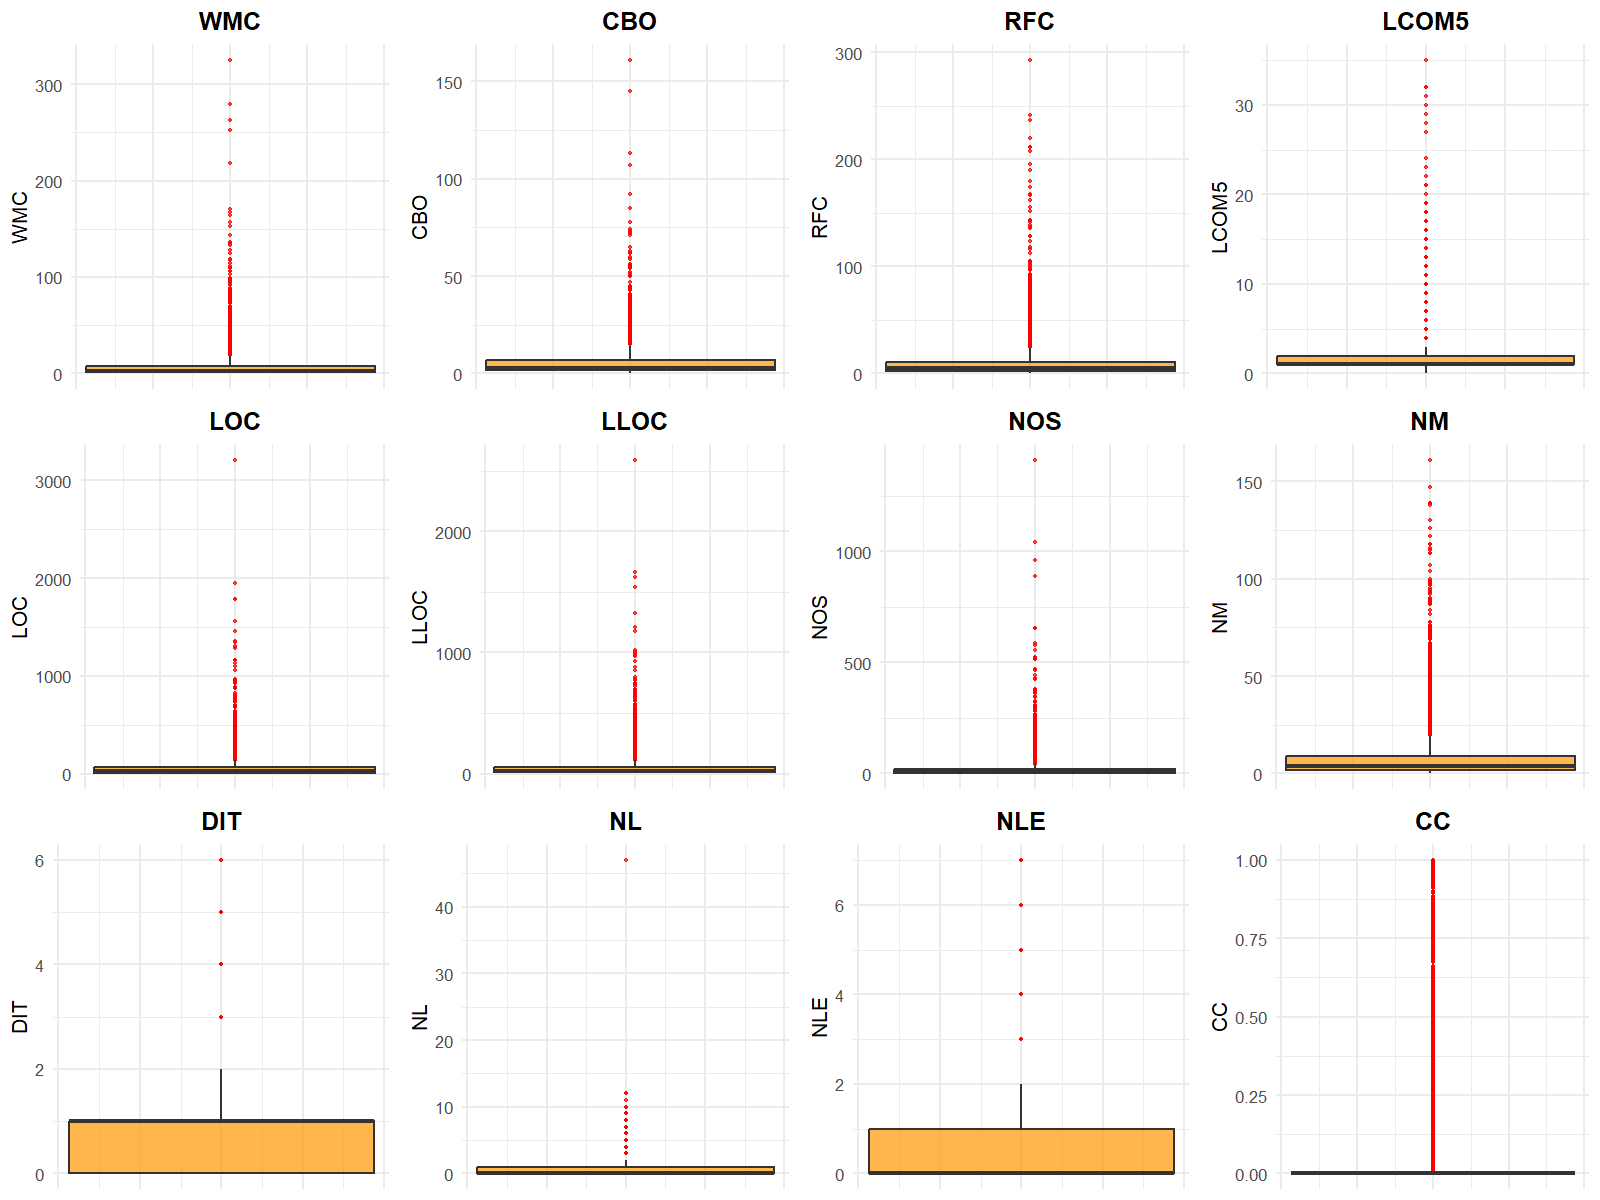
\includegraphics[width=0.95\textwidth]{../figuras/boxplots_class.png}
\caption{Boxplots das principais métricas --- Class-level}
\label{fig:boxplots_class}
\end{figure}

A Figura~\ref{fig:boxplots_class} evidencia a presença massiva de outliers em todas as métricas. A Tabela~\ref{tab:outliers} resume a detecção pelo método IQR. A proporção varia entre 5,86\% (NA) e 22,48\% (CC). Para métricas de tamanho (LOC, LLOC, NOS), $\approx$10\% são outliers, consistente com a regra de Pareto \cite{nagappan2006}. Os outliers não foram removidos por representarem classes legitimamente complexas. O File-level apresenta padrão análogo (McCC: 10,91\%; LLOC: 7,89\% de outliers).

\begin{table}[H]
\centering
\caption{Outliers pelo método IQR --- Class-level (seleção)}
\label{tab:outliers}
\footnotesize
\begin{tabular}{lrrr}
\toprule
\textbf{Variável} & \textbf{Outliers} & \textbf{\%} & \textbf{Limite Sup.} \\
\midrule
WMC  & 706   & 8,92  & 18,50 \\
CBO  & 644   & 8,13  & 14,50 \\
RFC  & 759   & 9,59  & 24,50 \\
LOC  & 799   & 10,09 & 140,00 \\
NOS  & 840   & 10,61 & 42,00 \\
NM   & 866   & 10,94 & 19,50 \\
CC   & 1.780 & 22,48 & 0,00 \\
\bottomrule
\end{tabular}
\end{table}

\subsection{Histogramas e Distribuições}

\begin{figure}[H]
\centering
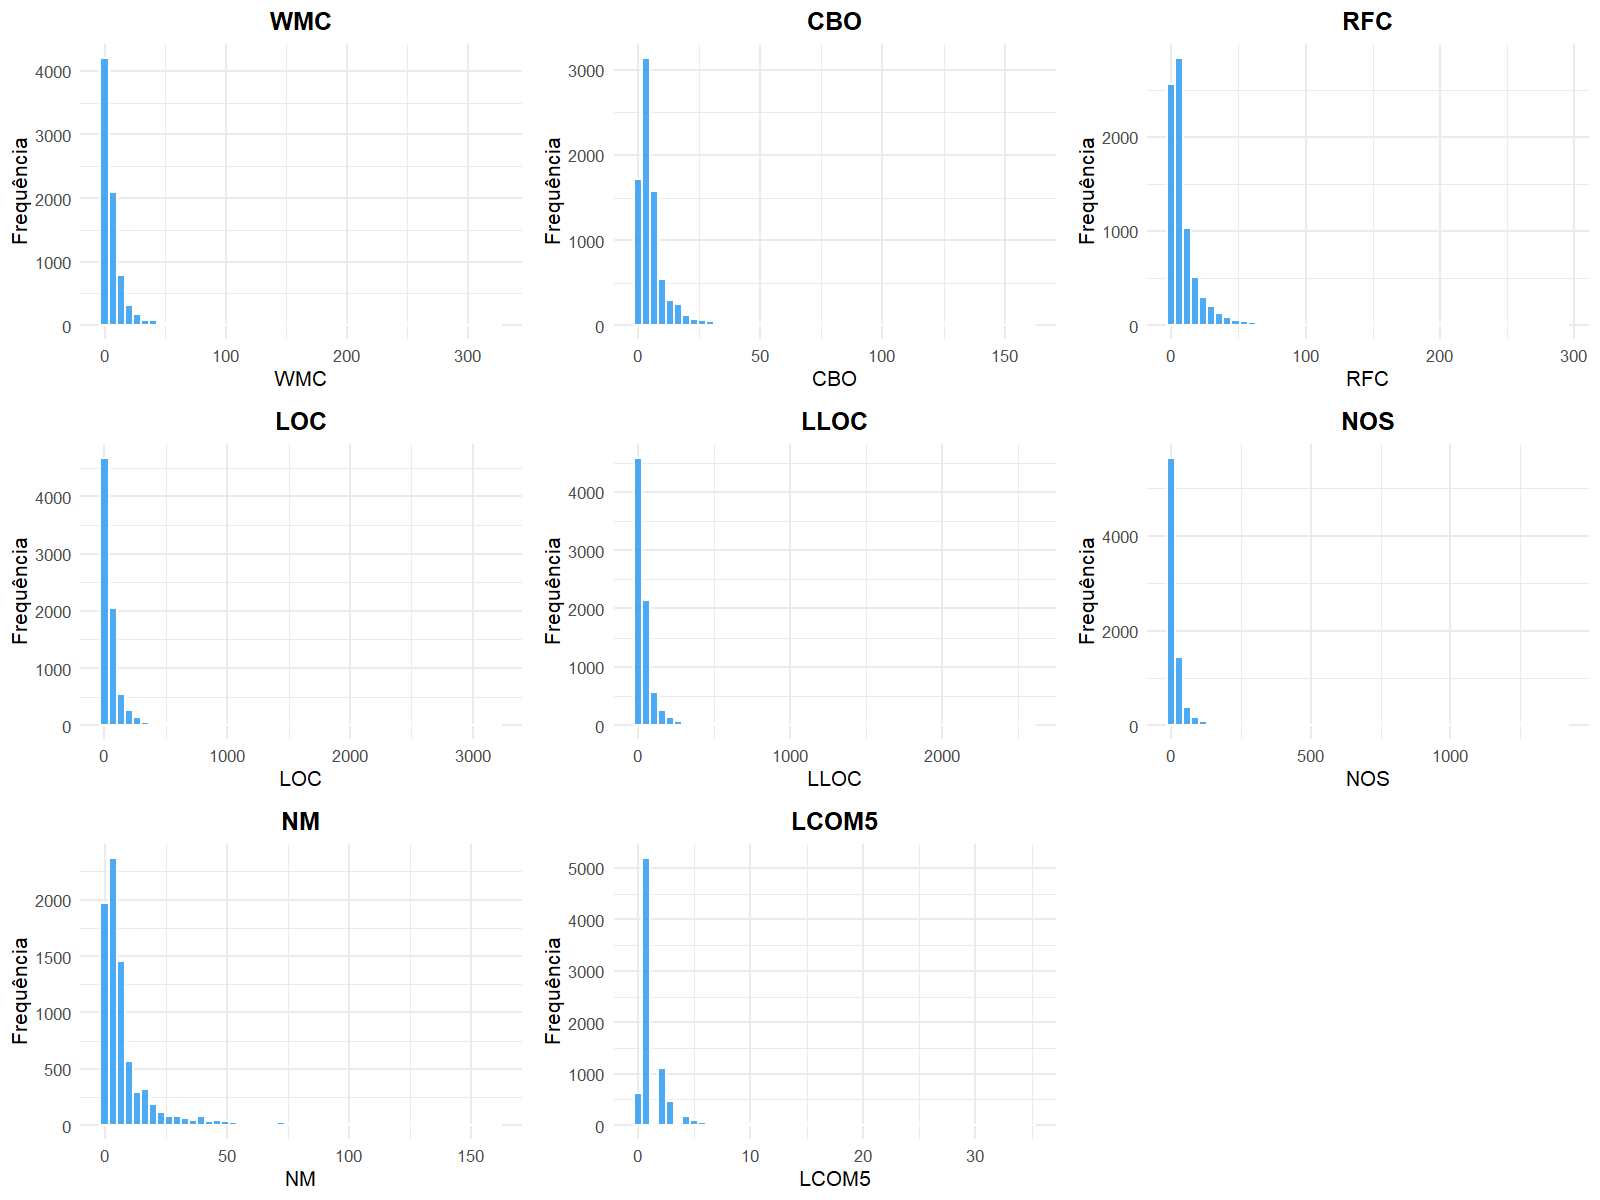
\includegraphics[width=0.95\textwidth]{../figuras/histogramas_class.png}
\caption{Histogramas das métricas Class-level}
\label{fig:hist_class}
\end{figure}

Os histogramas (Figura~\ref{fig:hist_class}) confirmam distribuições fortemente assimétricas à direita, com concentração massiva em valores baixos e caudas longas, comportamento esperado em métricas de software \cite{radjenovic2013}. A distribuição de bugs é extremamente desbalanceada: apenas 8 classes (0,10\%) e 6 arquivos (0,14\%) apresentam bugs registrados.

\subsection{Testes de Normalidade}

Para todas as variáveis, os testes de Shapiro-Wilk \cite{shapiro1965} e Lilliefors \cite{lilliefors1967} rejeitaram a hipótese nula de normalidade ($p < 10^{-50}$). A Tabela~\ref{tab:normalidade} apresenta estatísticas para variáveis representativas. Adotou-se Lilliefors em lugar do teste K-S com parâmetros estimados, que é anticonservativo \cite{lilliefors1967}. Para Shapiro-Wilk (limite de 5.000 obs.), utilizou-se amostra com seed=42.

\begin{table}[H]
\centering
\caption{Testes de normalidade --- Class-level}
\label{tab:normalidade}
\footnotesize
\begin{tabular}{lcccc}
\toprule
\textbf{Var.} & \textbf{SW} & \textbf{SW $p$} & \textbf{Lill. $D$} & \textbf{Lill. $p$} \\
\midrule
WMC & 0,421 & $< 10^{-83}$ & 0,308 & $< 2{,}2\!\times\!10^{-16}$ \\
CBO & 0,587 & $< 10^{-76}$ & 0,225 & $< 2{,}2\!\times\!10^{-16}$ \\
LOC & 0,424 & $< 10^{-83}$ & 0,311 & $< 2{,}2\!\times\!10^{-16}$ \\
DIT & 0,827 & $< 10^{-59}$ & 0,252 & $< 2{,}2\!\times\!10^{-16}$ \\
\bottomrule
\end{tabular}
\end{table}

A rejeição universal de normalidade justifica o uso de Spearman e implica cautela com métodos que assumem normalidade.

\subsection{Análise de Correlação}

Dado que todas as variáveis violam normalidade, complementou-se Pearson com Spearman (baseada em postos), mais robusta a outliers.

\begin{figure}[H]
\centering
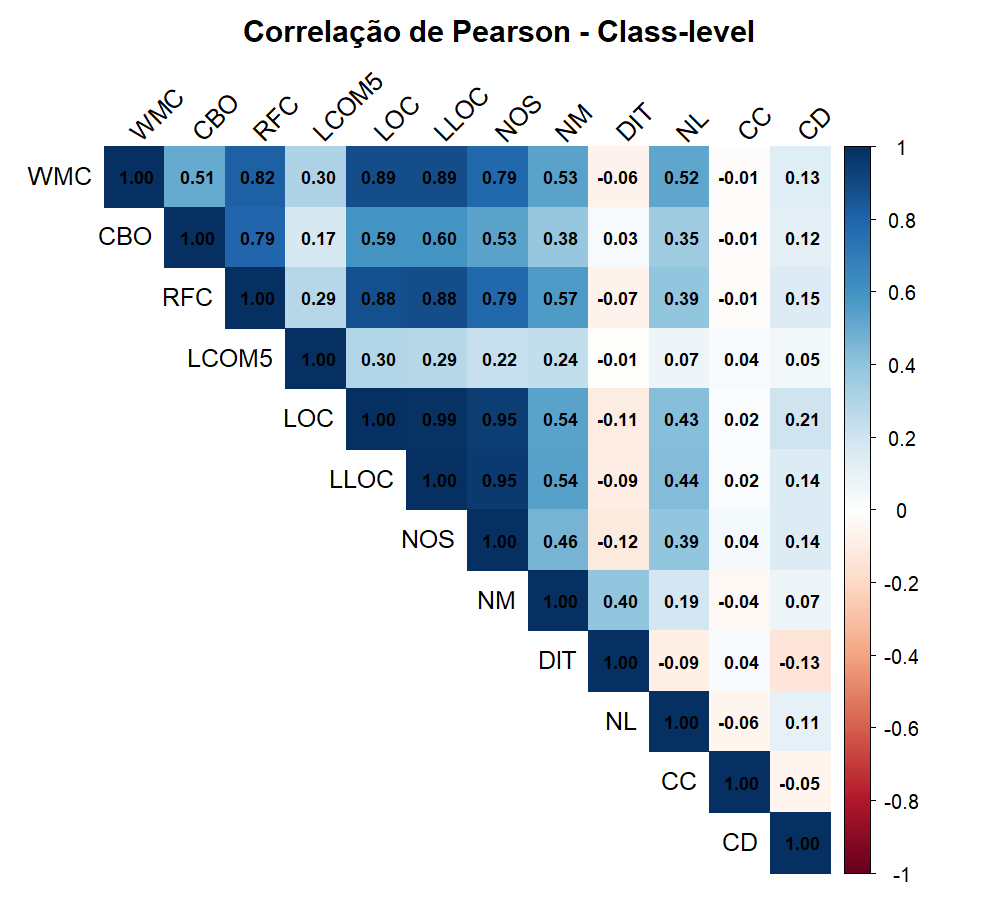
\includegraphics[width=0.80\textwidth]{../figuras/correlacao_heatmap_class.png}
\caption{Heatmap de correlação de Pearson --- Class-level}
\label{fig:corr_class}
\end{figure}

\textbf{Correlações fortes} ($|r| \geq 0{,}7$, Pearson): LOC$\times$LLOC: $r = 0{,}99$; LOC$\times$NOS: $r = 0{,}95$; WMC$\times$LOC: $r = 0{,}89$; WMC$\times$RFC: $r = 0{,}82$; CBO$\times$RFC: $r = 0{,}80$. \textbf{Moderadas} ($0{,}4 \leq |r| < 0{,}7$): WMC$\times$CBO: $r = 0{,}51$; CBO$\times$LOC: $r = 0{,}59$. As correlações de Spearman apresentam padrão semelhante com magnitudes geralmente mais elevadas (e.g., LOC$\times$LLOC: $\rho = 0{,}99$; NOS$\times$NL: $\rho = 0{,}72$). A convergência reforça a robustez dos achados.

\begin{figure}[H]
\centering
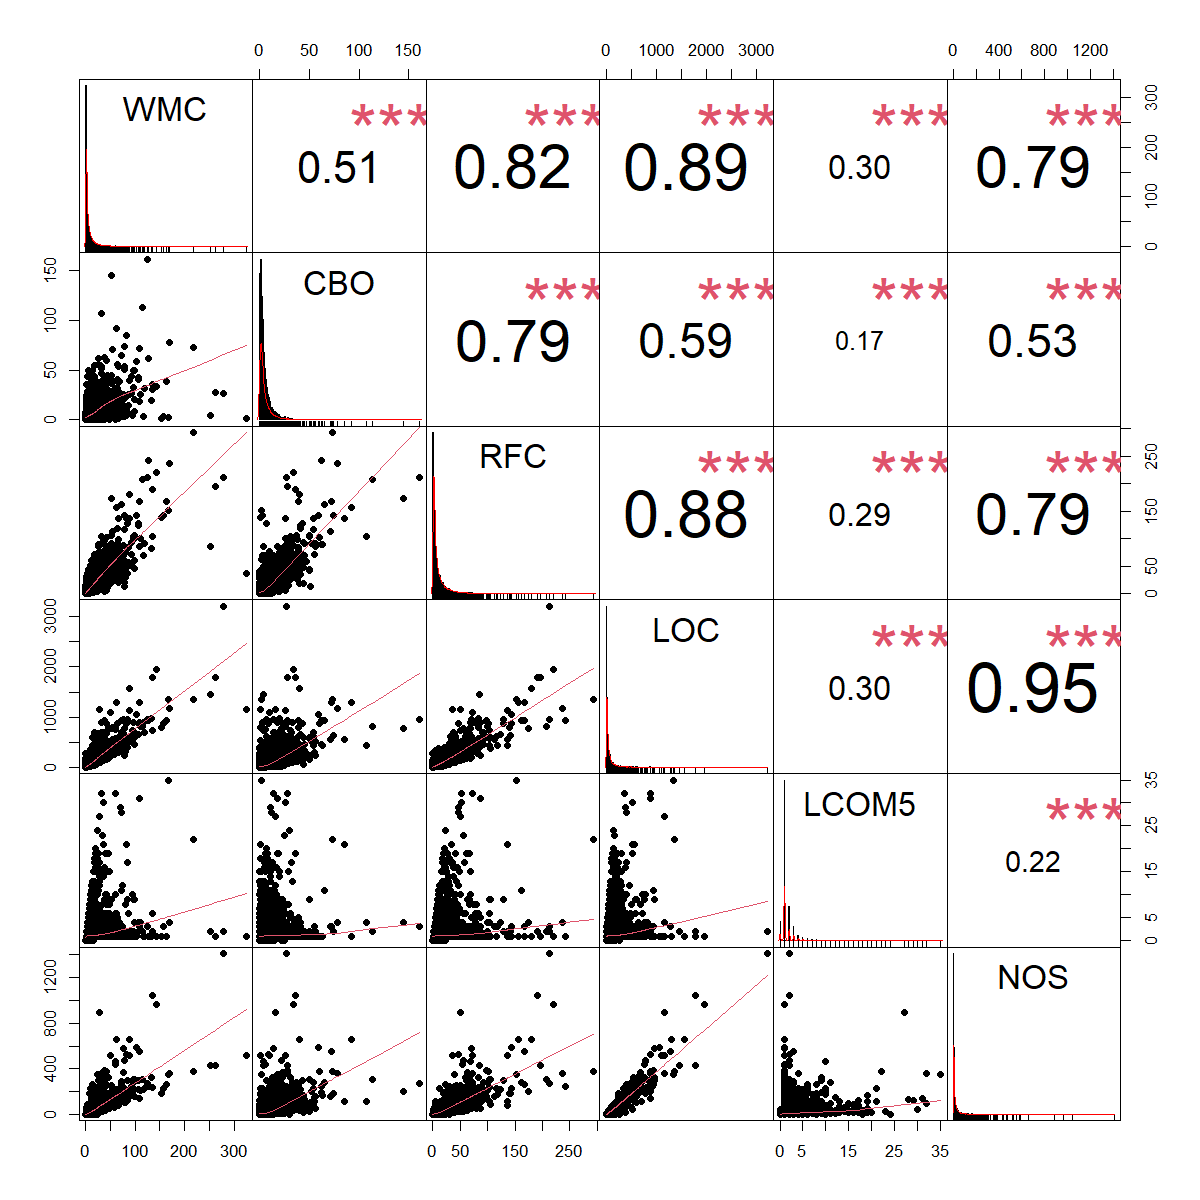
\includegraphics[width=0.80\textwidth]{../figuras/chart_correlation_class.png}
\caption{chart.Correlation --- métricas principais (Class-level)}
\label{fig:chart_corr}
\end{figure}

A Figura~\ref{fig:chart_corr} combina histogramas, dispersão e coeficientes de correlação. No File-level, as correlações mais fortes são McCC$\times$LLOC ($r = 0{,}72$) e ``N. previous modifications''$\times$``N. committers'' ($r = 0{,}77$; Spearman: $\rho = 0{,}90$).

\subsection{Análise de Multicolinearidade (VIF)}

Calculou-se o VIF para quantificar multicolinearidade \cite{montgomery2012}. No Class-level, RFC (VIF = 20,18), WMC (15,17) e LOC (10,98) excederam o limiar de 10. Após remoção iterativa de RFC, os VIF finais ficaram abaixo de 10 (WMC: 8,75; LOC: 9,16). No File-level, todos os VIF foram aceitáveis ($\leq$ 5,58).

\subsection{Regressão Logística}

Optou-se por regressão logística binária com pesos \textit{cost-sensitive} inversamente proporcionais à frequência de cada classe, evitando classificação trivial como classe majoritária.

\subsubsection{Modelo Class-level}

O modelo utilizou preditores remanescentes após remoção de VIF $>$ 10 (WMC, CBO, LOC, LCOM5, NL, DIT, CC). Os coeficientes apresentaram magnitude extrema (ordem $10^{12}$--$10^{15}$), indicando que o algoritmo \textit{não convergiu} --- separação completa dos dados, sintoma do desbalanceamento extremo (8 positivos em 7.917, EPV~$\approx$~1). O Pseudo $R^2$ (McFadden) foi $-10{,}76$ (modelo pior que o nulo). Na escala de McFadden, 0,2--0,4 indica ajuste excelente \cite{mcfadden1974}.

\subsubsection{Modelo File-level}

Os preditores foram McCC, LLOC, N.~previous modifications, N.~previous fixes, N.~committers e N.~developer commits. O Pseudo $R^2$ (McFadden) foi 0,59 (excelente), porém o algoritmo também não convergiu. Apenas LLOC não foi significativo ($p = 0{,}30$); os demais resultados devem ser interpretados com cautela dado o número ínfimo de positivos (6 instâncias).

\subsubsection{Métricas de Avaliação e Validação Cruzada}

\begin{table}[H]
\centering
\caption{Métricas de avaliação: regressão e validação cruzada (10-fold)}
\label{tab:metricas_avaliacao}
\footnotesize
\begin{tabular}{lrrrr}
\toprule
 & \multicolumn{2}{c}{\textbf{Treino completo}} & \multicolumn{2}{c}{\textbf{10-fold CV}} \\
\cmidrule(lr){2-3} \cmidrule(lr){4-5}
\textbf{Métrica} & \textbf{Class} & \textbf{File} & \textbf{Class} & \textbf{File} \\
\midrule
AUC-ROC   & 0,674 & 0,968 & 0,660 & 0,805 \\
AUC-PR    & 0,007 & 0,020 & ---   & ---   \\
Sensitivity & 0,375 & 1,000 & 0,625 & 0,833 \\
Precision   & 0,014 & 0,024 & 0,002 & 0,007 \\
F1-score    & 0,027 & 0,047 & 0,004 & 0,014 \\
Bal.~Acc.   & 0,674 & 0,972 & 0,664 & 0,836 \\
MCC         & 0,069 & 0,151 & 0,023 & 0,068 \\
\bottomrule
\end{tabular}
\end{table}

\begin{figure}[H]
\centering
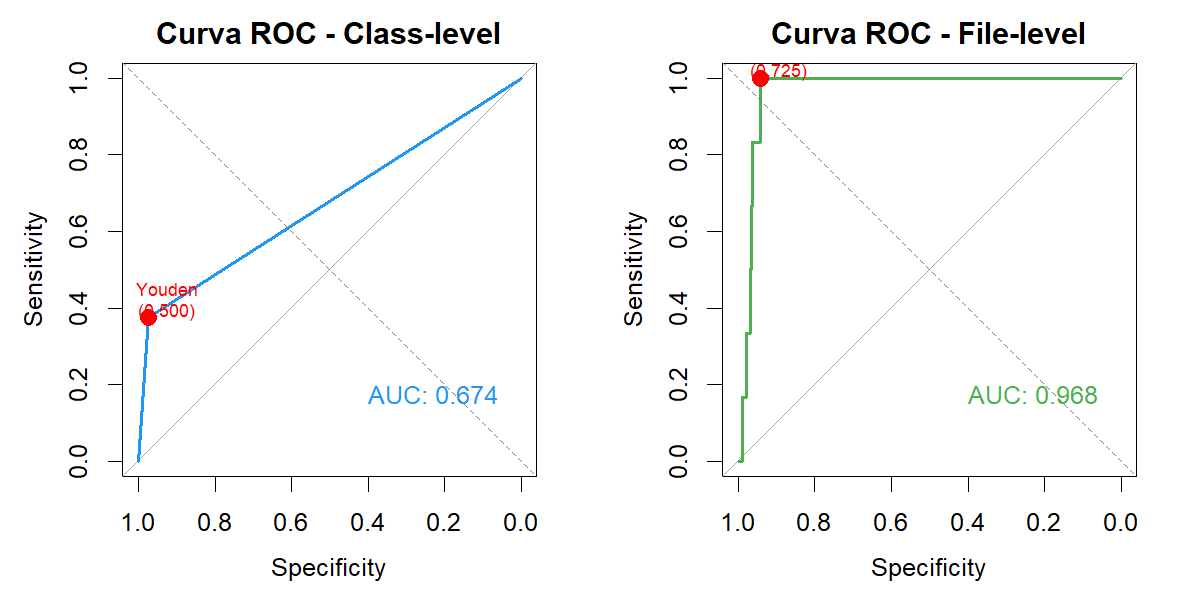
\includegraphics[width=0.95\textwidth]{../figuras/curva_roc.png}
\caption{Curvas ROC com Youden Index para Class e File-level}
\label{fig:roc}
\end{figure}

A Tabela~\ref{tab:metricas_avaliacao} consolida as métricas do treino completo e da validação cruzada estratificada com 10 folds. A degradação na CV confirma overfitting, especialmente no File-level (AUC: 0,97 $\to$ 0,81). Os valores de MCC próximos de zero (0,023 e 0,068) indicam poder preditivo praticamente nulo. A ``acurácia'' de 97--99\% é enganosa: um classificador trivial que sempre prediz ``sem bug'' obtém desempenho similar. As curvas Precision-Recall (não apresentadas por limitação de espaço) confirmam AUC-PR $\approx$ 0, reforçando a inadequação dos dados para predição.

\subsection{Discussão}

As métricas do Neo4j seguem distribuições fortemente assimétricas, consistente com a literatura \cite{radjenovic2013, gyimothy2005}. As correlações fortes entre LOC, LLOC, NOS, WMC e RFC indicam dimensões sobrepostas de tamanho e complexidade, confirmadas pela análise VIF. A correlação extremamente fraca entre métricas e bugs (máximo $r = 0{,}06$) contrasta com estudos anteriores \cite{basili1996, gyimothy2005}, explicável pelo desbalanceamento extremo e possível subreporte de defeitos.

Quanto às métricas CK: DIT e NOC possuem variância quase zero no Neo4j (design ``flat''), tornando-as pouco discriminativas. LCOM5 possui múltiplas definições na literatura, dificultando comparações entre estudos.

% =====================================================================
\subsection{Ameaças à Validade} \label{sec:ameacas}

\textbf{Interna:} (i) Desbalanceamento extremo da variável alvo (8 e 6 positivos; EPV $\approx$ 1, muito abaixo do mínimo de 10 \cite{hosmer2013}); (ii) Teste K-S original com parâmetros estimados foi anticonservativo --- corrigido com Lilliefors; (iii) Multicolinearidade severa (LOC$\times$LLOC: $r = 0{,}99$) --- corrigida via VIF; (iv) Modelo avaliado no conjunto de treino --- corrigido com 10-fold CV.

\textbf{Externa:} Resultados específicos ao Neo4j; dataset de versão única; possível viés de seleção do GitHub Bug Dataset.

\textbf{Construto:} Métricas CK são proxies imperfeitos de qualidade; ``Number of bugs'' depende da completude do rastreamento; DIT e NOC com variância quase zero são irrelevantes neste contexto.

% =====================================================================
\section{Conclusão} \label{sec:conclusao}

Apresentou-se uma análise estatística de métricas do Neo4j (GitHub Bug Dataset v1.1) com testes de normalidade corrigidos (Lilliefors), correlação de Pearson e Spearman, análise VIF, regressão \textit{cost-sensitive} e validação cruzada. Todas as métricas seguem distribuições assimétricas com correlações fortes entre tamanho e complexidade (LOC$\times$LLOC: $r = 0{,}99$). O principal achado é a \textbf{inadequação do dataset para predição de defeitos}: com EPV~$\approx$~1, os modelos são não confiáveis e a ``alta acurácia'' é enganosa.

Como trabalhos futuros: (i) combinar múltiplas versões do Neo4j para aumentar instâncias positivas; (ii) aplicar \textit{Random Forest} ou \textit{gradient boosting}; (iii) explorar \textit{cross-project defect prediction}.

% =====================================================================
\bibliographystyle{plain}
\bibliography{sbc-template}

\end{document}
